\documentclass{zusammenfassung}
\usepackage{array}
\usepackage{booktabs}
\usepackage{color}
\usepackage{colortbl}
\usepackage{xstring}
\usepackage{intcalc}
\usepackage{alphalph}
\usepackage[misc]{ifsym}
\graphicspath{ {./illustrationen/} }
\setmonofont{Linux Libertine Mono}
\usetikzlibrary{matrix}

\begin{document}
\maketitle{Klasse 6/7}{10. Februar 2015}{2014/2015}

Die sogenannte \emph{Skytale} ist das älteste bekannte Verschlüsselungsverfahren und stammt aus der Zeit um 500 v.~Chr. In Sparta
wurde damals ein Streifen Pergament oder Leder um einen Holzstab mit festem Durchmesser gewickelt. Die Nachricht, die geheim
gehalten werden sollte (der sogennante \emph{Klartext}) wurde längs des Stabs auf das Pergament geschrieben. Beim Abwickeln ergab
sich nur noch eine Folge von durcheinandergewürfelten Buchstaben, der \emph{Geheimtext}. Beim Entschlüsseln wurde das Band auf
eine Skytale des selben Durchmessers gewickelt und konnte so wieder gelesen werden.

Man kann dieses Verschlüsselungsverfahren auch beschreiben, wenn man keine Holzstäbe zur Hand hat. Der geheime \emph{Schlüssel}
des Verschlüsselungsverfahrens ist der Umfang des Holzstabs, gemessen als Anzahl der Buchstaben $n$, die einmal um den Stab
passen. Man verschlüsselt nun, indem man den Text zeilenweise in $n$ Zeilen schreibt. Der Geheimtext ergibt sich, indem man
spaltenweise liest. Entschlüsselt wird, indem man einen Text spaltenweise in $n$ Zeilen schreibt und zeilenweise liest.

Das sogenannte \emph{Kerckhoffs'sche Prinzip} in der Kryptographie besagt, dass die Sicherheit eines Verschlüsselungsverfahrens nur
auf der Geheimhaltung des Schlüssels, nicht aber auf der Geheimhaltung des Verschlüsselungsverfahrens beruht. In der heutigen Zeit
sprechen viele Gründe für das Kerckhoffs'sche Prinzip. Die wichtigsten beiden sind folgende:
Erstens bestehen die Algorithmen aus deutlich mehr Information als der
Schlüssel und können daher schwerer geheimgehalten werden. Zweitens werden Fehler in öffentlichen Verfahren leichter entdeckt als
in nicht-öffentlichen, da sich mehr Menschen damit befassen.

Akzeptiert man das Kerckhoffs'sche Prinzip (was wir tun werden), dann ist die Skytale kein sehr sicheres
Verschlüsselungsverfahren. Ein wesentlicher Grund dafür ist, dass die Anzahl der möglichen Schlüssel sehr klein sind: Als
Schlüssel kommen nur Zahlen zwischen $1$ und der Länge des Textes in Frage. Also kann man relativ schnell alle möglichen Schlüssel
durchprobieren.

Ein Beispiel: Wir haben folgenden Text gegeben, von dem wir wissen, dass er mit einer Skytale verschlüsselt wurde:

\def\mytext{DEEHETARIRIESINGMXHSSEETITEHR}
\StrLen{\mytext}[\len]
\begin{center}
  \begin{tikzpicture}
    \foreach\i in {1,...,\len} {
      \node at (\i/2,0) {\StrMid{\mytext}{\i}{\i}};
    }
  \end{tikzpicture}
\end{center}

Wir können jetzt ausprobieren, welche Längen in Frage kommen. Länge $2$ würde den Anfang "`DEEA..."' ergeben; das kann nicht sein.
Bei Länge $3$ hat man "`DH..."', für Länge $4$ "`DEISM..."'. Länge $5$ ergibt "`DT..."', für Länge $6$ hätte man "`DASHIERI..."'.
Das klingt schon nach einem vernünftigen Beginn. Jetzt kann man den Text einmal probehalber mit Länge $6$ entschlüsseln und erhält
tatsächlich die Nachricht

\begin{center}
  \begin{tikzpicture}[x=0.5cm,y=-0.5cm]
    \foreach\i in {1,...,\len} {
      \node at (\intcalcDiv{\intcalcDec{\i}}{6},\intcalcMod{\intcalcDec{\i}}{6}) {\StrMid{\mytext}{\i}{\i}};
    }
  \end{tikzpicture}
\end{center}

Auch längere Texte können so relativ leicht entschlüsselt werden.

Ein zweites schon in der Antike bekanntes Verfahren ist die \emph{Cäsar-Verschlüsselung}. Hier wird jeder Buchstabe des Alphabets
durch einen Buchstaben, der drei Plätze weiter hinten im Alphabet liegt, ersetzt. Dabei ist die Zahl $3$ ziemlich willkürlich;
allgemeiner kann man als Cäsar-Verschlüsselung das folgende Verfahren bezeichnen: Der geheime Schlüssel ist ein Buchstabe. Zum
Verschlüsseln und Entschlüsseln schreibt man das Alphabet zweimal untereinander, einmal normal und einmal beginnend mit dem
Schlüsselbuchstabe. Ist der Schlüsselbuchstabe beispielsweise D wie in der ursprünglichen Cäsar-Verschlüsselung, dann sieht das
folgendermaßen aus:

\begin{center}
  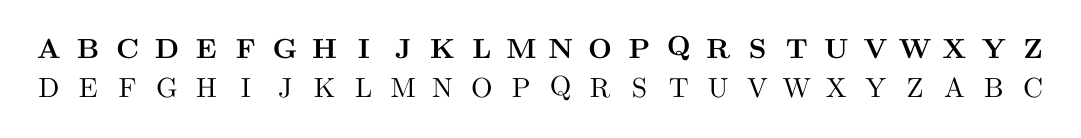
\begin{tikzpicture}[x=0.5cm,y=-0.5cm]
    \foreach\x in {1,...,26}{
      \node at (\x,0) {\bf\AlphAlph{\x}};
      \node at (\x,1) {\AlphAlph{\intcalcInc{\intcalcMod{\intcalcAdd{\x}{2}}{26}}}};
    }
  \end{tikzpicture}
\end{center}

Die Verschlüsselung erfolgt, indem jeder Buchstabe aus dem Text durch den darunterstehenden Buchstaben ersetzt wird. Um den so
entstandenen Geheimtext wieder zu entschlüsseln, muss man die Buchstaben von unten nach oben ersetzen.

Diese Art von Verschlüsselung ist ein Spezialfall der sogenannten \emph{monoalphabetischen Substitution}. Dabei ist der Schlüssel
ein beliebiges Zeichen für jeden Buchstaben des Alphabets. Die Ver- und Entschlüsselung funktioniert wieder wie bei der
Cäsar-Verschlüsselung. Ein Beispiel wäre folgendes:

\begin{center}
  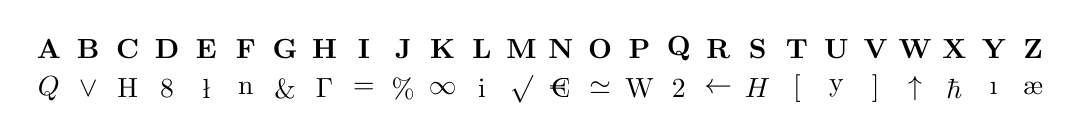
\begin{tikzpicture}[x=0.5cm,y=-0.5cm]
    \foreach\x in {1,...,26}{
      \node at (\x,0) {\bf\AlphAlph{\x}};
    }
    \foreach\x/\txt in {1/$\mathbb Q$,2/$\vee$,3/H,4/8,5/\l,6/n,7/\&,8/$\Gamma$,9/=,10/\%,11/$\infty$,12/i,
      13/$\sqrt{}$,14/€,15/$\simeq$,16/W,17/2,18/$\leftarrow$,19/$\mathbb H$,20/[,21/y,22/],23/$\uparrow$,24/$\hbar$,
      25/\i,26/\ae} {
      \node at (\x,1) {\txt};
    }
  \end{tikzpicture}
\end{center}

Eine etwas praktischere Form ist die sogenannte \emph{Schlüsselwort-Methode}. Hier ist der Schlüssel die Kombination aus einem
Schlüsselbuchstaben und einem Schlüsselwort. Das Schlüsselwort wird jetzt, beginnend unter dem Schlüsselbuchstaben, unter das
ursprüngliche Alphabet geschrieben. Dabei werden Buchstaben, die im Schlüsselwort mehrfach vorkommen, nur einmal aufgeschrieben.
Unter das restliche Alphabet werden jetzt die Buchstaben des Alphabets in der üblichen Reihenfolge untereinander geschrieben, 
wobei die Buchstaben des Schlüsselworts ausgelassen werden.
Besteht der Schlüssel beispielsweise aus dem Schlüsselwort "`Handcreme"' und dem Schlüsselbuchstaben F, dann sieht das
Verschlüsselungsschema folgendermaßen aus:

\begin{center}
  \def\secret{VWXYZHANDCREMBFGIJKLOPQSTU}
  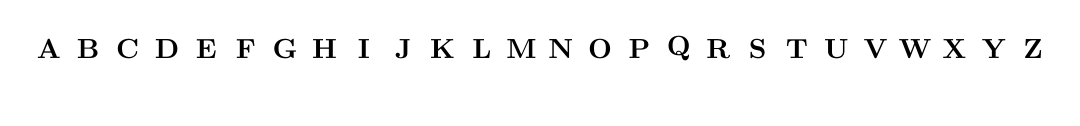
\begin{tikzpicture}[x=0.5cm,y=-0.5cm]
    \foreach\x in {1,...,26}{
      \node at (\x,0) {\bf\AlphAlph{\x}};
      \node at (\x,1) {\StrMid{\secret}{\x}{\x}};
    }
  \end{tikzpicture}
\end{center}

Die Cäsar-Verschlüsselung kann wieder leicht durch Ausprobieren geknackt werden, da es nicht sehr viele Schlüssel gibt. Aber auch
andere monoalphabetische Substitutionsmethoden können ohne Kenntnis des Schlüssels vergleichsweise einfach entschlüsselt werden.
Dazu verwendet man, dass nicht alle Buchstaben in deutschen Texten mit denselben Häufigkeiten auftreten. Beispielsweise ist das E
mit einem Anteil von über $17$ Prozent der mit Abstand häufigste Buchstabe, gefolgt vom N mit knapp $10$ Prozent. Das Zeichen, das
im Geheimtext also am Häufigsten vorkommt, entspricht mit hoher Wahrscheinlichkeit dem E, und die Zeichen mit den nächstmeisten
Häufigkeiten dürften den Buchstaben N, I, S, R, A und T entsprechen (möglicherweise aber nicht genau in dieser Reihenfolge, da die
Häufigkeiten dieser Buchstaben recht nahe beieinander liegen). Oft kann man jetzt schon weitere Buchstaben erraten und so den Text
entschlüsseln.

Ein Verschlüsselungsverfahren, das diesem Mangel abhilft, ist die \emph{homophone Chiffre}. Hier werden Buchstaben nicht immer mit
demselben Zeichen verschlüsselt, sondern jeder Buchstabe bekommt mehrere Zeichen, je nach seiner Häufigkeit. Beispielsweise kann
man als Geheimtext-"`Alphabet"' alle zweistelligen Ziffernfolgen von 00 mit 99 nehmen. Da das E in der deutschen Sprache vier mal 
so häufig vorkommt wie das U, werden dem E auch viermal so viele Ziffernfolgen zugeteilt.

Allerdings kann auch die homophone Chiffre geknackt werden, wenn man die Häufigkeit von Buchstabenpaaren betrachtet: Manche
Buchstabenpaare sind deutlich häufiger als andere, was als Ansatz zur Analyse eines Geheimtextes verwendet werden kann.

Ein anderer Ansatz, bei dem gleiche Buchstaben nicht immer mit dem gleichen Zeichen verschlüsselt werden, ist die sogenannte
\emph{Vigenère-Verschlüsselung}. Der Schlüssel ist hier ein Wort. Dieses Wort wird -- immer wiederholt -- über den Klartext 
geschrieben. Ist beispielsweise das Wort "`Kaugummi"', dann sieht das Schema folgendermaßen aus:

\begin{center}
  \def\secret{KAU GUMM IKAU GUMM IKAUGUM MIK AUGUMMI KAUGUM}
  \def\text{MAN KANN FUER JEDE LOESUNG EIN PROBLEM FINDEN.}
  \begin{tikzpicture}[x=0.32cm,y=-0.5cm,every node/.style={anchor=base}]
    \foreach\x in {1,...,46}{
      \node at (\x,0) {\StrMid{\secret}{\x}{\x}};
      \node at (\x,1) {\bf\StrMid{\text}{\x}{\x}};
    }
  \end{tikzpicture}
\end{center}

Nun verschlüsselt man jeden Buchstaben mit der Cäsar-Verschlüsselung, wobei man als Schlüsselbuchstabe den
Buchstaben nimmt, der direkt drüber steht. Also verschlüsselt man das erste M mit der Cäsar-Verschlüsselung zum Buchstaben K, das
A mit Cäsar-Verschlüsselung mit Buchstabe A und so weiter.

Der Text von oben würde dann als 

\begin{center}
  \def\text{WAH EMZV FOKL VMNE RIQECXG KCZ XBOVRYY NSNXKH.}
  \begin{tikzpicture}[x=0.32cm,y=-0.5cm,every node/.style={anchor=base}]
    \foreach\x in {1,...,46}{
      \node at (\x,0) {\StrMid{\text}{\x}{\x}};
    }
  \end{tikzpicture}
\end{center}

verschlüsselt werden. Doch selbst dieser raffinierte Verschlüsselungsmechanismus kann geknackt werden. Der wesentliche Schritt 
dabei ist, die Länge des Schlüsselworts zu bestimmen. Kennt man nämlich bereits die Länge des Schlüsselworts, dann kann man eine
Häufigkeitsanalyse für die Teilportionen durchführen. Weiß man beispielsweise, dass das gewählte Schlüsselwort die Länge $4$ hat,
dann kann man die Buchstaben des Geheimtexts in vier Portionen aufteilen: Diejenigen, die mit dem ersten Buchstaben verschlüsselt
wurden, diejenigen, die mit dem zweiten Buchstaben verschlüsselt wurden, und so fort. Bei jedem dieser Stapel zählt man die
Buchstabenhäufigkeiten. Der häufigste Buchstabe ist dann wieder mit großer Wahrscheinlichkeit der Buchstabe, der für das E steht,
und der nächsthäufige steht möglicherweise für das N. Falls die Texte nicht sehr lang sind, muss das zwar nicht immer der Fall
sein, aber oft kommt man durch genaues Vergleichen trotzdem sehr bald auf die richtige Lösung.

Die erste Methode, um die Schlüssellänge zu bestimmen, ist der sogenannte \emph{Kasiski-Test}. Er lässt sich am Besten anhand
eines Beispiels beschreiben:

\begin{center}
  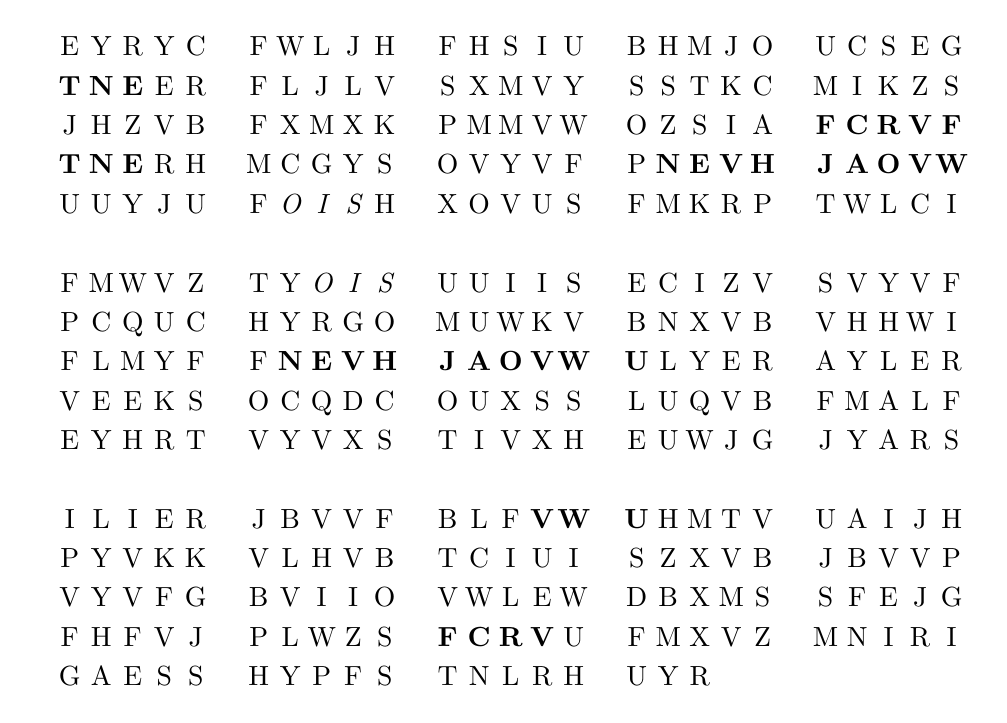
\begin{tikzpicture}[x=0.4cm,y=-0.5cm,every node/.style={anchor=base}]
    \def\putText#1#2#3{%
      \StrLen{#1}[\len]%
      \edef\xa{#2}%
      \edef\xb{\intcalcAdd{#2}{\len}}%
      \foreach\x in {\xa,...,\xb} {\node at (\x+\intcalcDiv{\intcalcDec{\x}}{5},#3)%
        {\StrMid{#1}{\intcalcSub{\x}{\xa}}{\intcalcSub{\x}{\xa}}}; }%
    }
    \putText{EYRYCFWLJHFHSIUBHMJOUCSEG}{0}{0}
    \putText{ERFLJLVSXMVYSSTKCMIKZS}{3}{1} {\bf\putText{TNE}{0}{1}}
    \putText{JHZVBFXMXKPMMVWOZSIA}{0}{2} {\bf\putText{FCRVF}{20}{2}}
    \putText{RHMCGYSOVYVFP}{3}{3} {\bf\putText{TNE}{0}{3} \putText{NEVHJAOVW}{16}{3}}
    \putText{UUYJUF}{0}{4} {\it\putText{OIS}{6}{4}} \putText{HXOVUSFMKRPTWLCI}{9}{4}
    \putText{FMWVZTY}{0}{6} {\it\putText{OIS}{7}{6}} \putText{UUIISECIZVSVYVF}{10}{6}
    \putText{PCQUCHYRGOMUWKVBNXVBVHHWI}{0}{7}
    \putText{FLMYFF}{0}{8} {\bf\putText{NEVHJAOVWU}{6}{8}} \putText{LYERAYLER}{16}{8}
    \putText{VEEKSOCQDCOUXSSLUQVBFMALF}{0}{9}
    \putText{EYHRTVYVXSTIVXHEUWJGJYARS}{0}{10}
    \putText{ILIERJBVVFBLF}{0}{12} {\bf\putText{VWU}{13}{12}} \putText{HMTVUAIJH}{16}{12}
    \putText{PYVKKVLHVBTCIUISZXVBJBVVP}{0}{13}
    \putText{VYVFGBVIIOVWLEWDBXMSSFEJG}{0}{14}
    \putText{FHFVJPLWZS}{0}{15} {\bf\putText{FCRV}{10}{15}} \putText{UFMXVZMNIRI}{14}{15}
    \putText{GAESSHYPFSTNLRHUYR}{0}{16}
  \end{tikzpicture}
\end{center}

Hier sieht man einige Zeichenfolgen, die mehrfach vorkommen. Höchstwahrscheinlich entstehen solche Zeichenfolgen, indem dieselbe
Zeichenfolge im Originaltext mit denselben Schlüsselbuchstaben verschlüsselt wird. Das ist nur dann der Fall, wenn der Abstand
zwischen zwei Vorkommnissen der Zeichenfolgen ein Vielfaches der Schlüssellänge ist. Man kann also die Abstände zwischen den
mehrfach vorkommenden Zeichenfolgen bestimmen und ihren größten gemeinsamen Teiler berechnen, Dieser Wert oder ein Teiler von
diesem Wert wird höchstwahrscheinlich die Schlüssellänge sein. Im Beispiel ergibt sich:

\begin{center}
  \begin{tabular}{ccc}
    \toprule
    \bf Folge&\bf Abstand&\bf Primfaktorzerlegung\\
    \midrule
    TNE&50&$2\cdot 5^2$\\
    FCRV&265&$5\cdot 53$\\
    NEVHJAOVWU&90&$2\cdot 3^2\cdot 5$\\
    VWU&75&$3\cdot 5^2$\\
    \bottomrule
  \end{tabular}
\end{center}

Der größte gemeinsame Teiler der Abstände ist in diesem Fall $5$. Allerdings kann auch etwas schiefgehen: Beispielsweise kommt
zweimal im Text die Buchstabenfolge OIS vor, und zwar mit einem Abstand von $26=2\cdot 13$. Zählt man das dazu, dann wäre der
größte gemeinsame Teiler $1$, es würde sich also um eine normale Cäsar-Verschlüsselung handeln. Dass das nicht der Fall ist
überprüft man leicht. Solche Ausreißer kann es immer geben; allerdings ist es extrem unwahrscheinlich, dass so eine lange
Zeichenkette wie NEVHJAOVWU einen Ausreißer darstellt.

Ein Nachteil dieser Methode ist, dass man die Schlüsselwortlänge nur bis auf Teiler und Vielfache ausrechnen kann. Die nächste
Methode liefert eine Größenordnung für die Schlüsselwortlänge; mit der Kombination aus beiden bekommt man zumindest bei längeren
Texten sehr wahrscheinlich das richtige Ergebnis für die Schlüsselwortlänge. Diese zweite Methode ist der \emph{Friedman-Test}. Er
besteht aus zwei auf den ersten Blick kompliziert aussehenden Formeln:

\begin{table}[h]
  \caption{Formeln für den Friedman-Test}
  \begin{center}
    \begin{align*}
      I&=\frac{\sum_{i=1}^{26}n_i(n_i-1)}{n(n-1)}\tag{Koinzidenzindex}\\
      h&=\frac{0{,}0377n}{I(n-1)-0{,}0385n+0{,}0762}\tag{Schlüsselwortlänge}
    \end{align*}
  \end{center}
\end{table}

Mit der ersten Formel wird der sogenannte \emph{Koinzidenzindex} des Textes berechnet. Das ist die Wahrscheinlichkeit dafür, dass
zwei zufällig herausgegriffene Buchstaben aus dem Text gleich sind. Dabei sind die Zahlen $n_1,n_2,n_3,\ldots$ die Anzahlen des
ersten Buchstabens (A), des zweiten Buchstabens (B), des dritten Buchstabens (C) und so weiter. Das Symbol $\sum_{i=1}^{26}$
bedeutet, dass man über die Werte von $n_i(n_i-1)$ summieren soll, wobei $i$ jede Zahl zwischen $1$ und $26$ einmal annimmt. Der
Nenner des Bruchs ist also einfach eine Abkürzung:

\[
  \sum_{i=1}^{26}n_i(n_i-1)=n_1\cdot(n_1-1)+n_2\cdot(n_2-1)+n_3\cdot(n_3-1)+\cdots.
\]

Das Symbol $n$ im Nenner ist die Anzahl der Buchstaben des Textes. Um also den Koinzidenzindex zu berechnen, zählt man mit einer
Strichliste die Häufigkeiten jedes Buchstabens, also die Zahlen $n_1,n_2,\ldots$, und berechnet dann daraus die Zahlen
$n_1(n_1-1),n_2(n_2-1),n_3(n_3-1),\ldots$. Diese Zahlen werden alle addiert und das Ergebnis durch $n(n-1)$ geteilt. Ein Beispiel,
bei dem nur die Buchstaben A, B, C und D vorkommen, wäre folgendes:

\begin{center}
  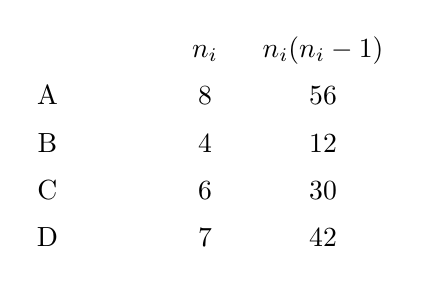
\begin{tikzpicture}[x=1cm,y=-0.6cm,every node/.style={anchor=base}]
    \node at (2,-1) {$n_i$};
    \node at (3.5,-1) {$n_i(n_i-1)$};
    \node at (0,0) {A};
    \node at (1,0) {\StrokeFive\StrokeThree};
    \node at (2,0) {8};
    \node at (3.5,0) {56};
    \node at (0,1) {B};
    \node at (1,1) {\StrokeFour};
    \node at (2,1) {4};
    \node at (3.5,1) {12};
    \node at (0,2) {C};
    \node at (1,2) {\StrokeFive\StrokeOne};
    \node at (2,2) {6};
    \node at (3.5,2) {30};
    \node at (0,3) {D};
    \node at (1,3) {\StrokeFive\StrokeTwo};
    \node at (2,3) {7};
    \node at (3.5,3) {42};
  \end{tikzpicture}
\end{center}

Die Summe im Zähler der Formel für $I$ ist dann $56+12+30+42=140$. Die Zahl $n$ ergibt sich als Summe der einzelnen
Buchstabenhäufigkeiten, also $n=8+4+6+7=25$, und daher $n(n-1)=25\cdot 24=600$. Insgesamt ist in diesem Fall also

\[
  I=\frac{140}{600}=\frac{7}{30}\approx 0{,}23333333.
\]

Jetzt kann man die Zahlen $I$ und $n$ in die zweite Formel einsetzen und erhält für die Schlüssellänge

\[
  h=\frac{0{,}0377\cdot 25}{0{,}2333333\cdot 24-0{,}0385\cdot 25+0{,}0762}=\frac{0{,}9425}{4.7136992}\approx 0.1999.
\]

Das zeigt auch gleich, dass unser Beispiel nicht sehr realistisch ist, da die Häufigkeiten der einzelnen Buchstaben stark
voneinander abweichen (22 Buchstaben kommen kein einziges Mal vor, das A dagegen sogar 8 Mal!). Allerdings zeigt das Beispiel auch
gleich zwei Schwachstellen des Friedman-Tests: Erstens kommt mit hoher Wahrscheinlichkeit bei dem Test keine ganze Zahl als
Ergebnis heraus, und zweitens muss das Ergebnis nicht unbedingt stimmen; es stimmt nur \emph{wahrscheinlich} relativ gut, und die
Wahrscheinlichkeit dafür, dass es gut stimmt, steigt mit der Gesamtlänge des Textes. Eine Schlüssellänge von etwa $\frac 15$ ist
jedenfalls sicher nicht möglich.

\end{document}
